
\begin{SCfigure*}
	\centering
	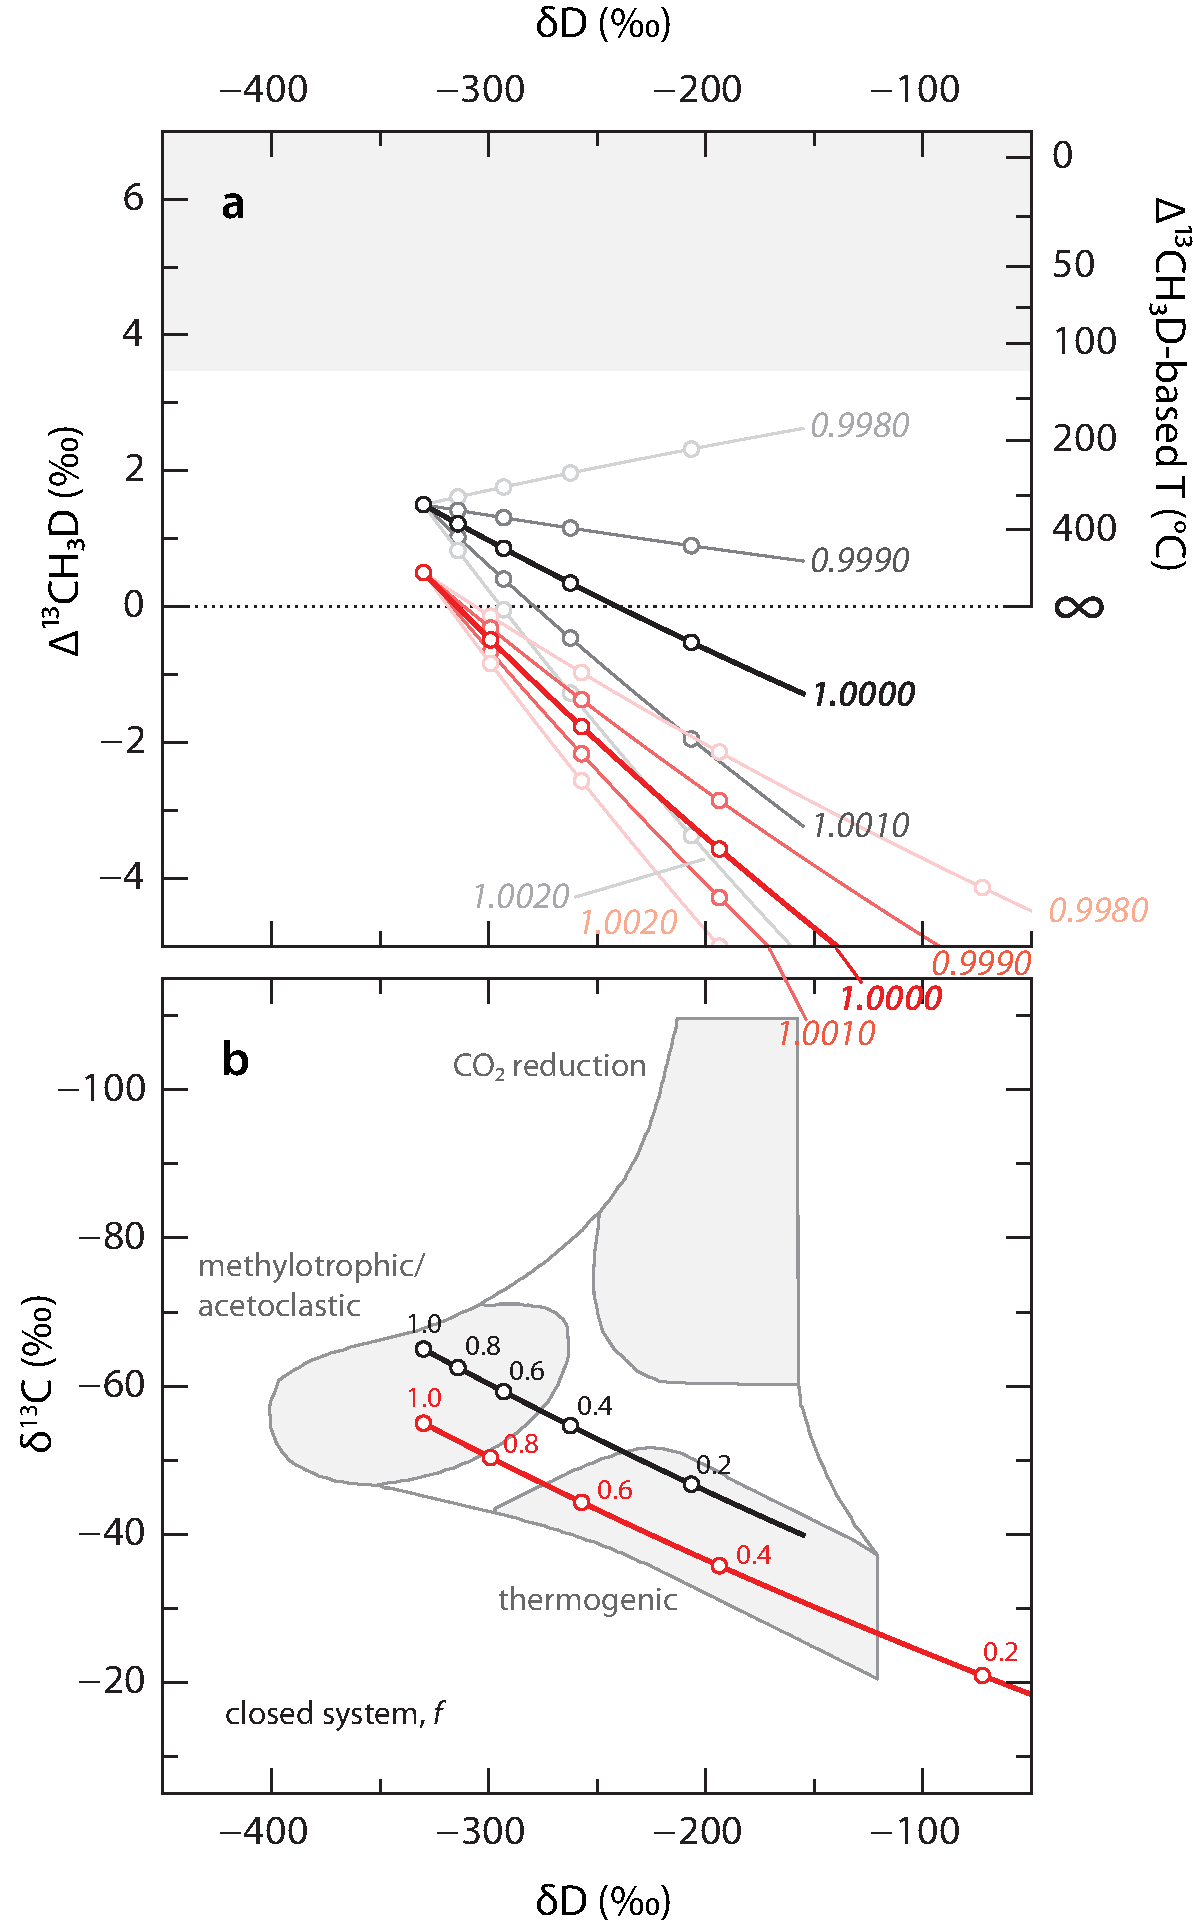
\includegraphics[width=0.5\textwidth]{figures/Fig4.3}
	\caption[Trajectories for isotope/isotopologue ratios of methane oxidized in a closed system]{Modeled changes in \textbf{(a)}
		Δ\textsuperscript{13}CH\textsubscript{3}D vs.\ δD and \textbf{(b)}
		δ\textsuperscript{13}C vs.\ δD of residual methane during aerobic methane
		oxidation under closed system conditions. Solid lines represent model
		predictions (from \mrefs[]{Eqns.}{eqn:4:13}, \ref{eqn:4:16}, and~\ref{eqn:4:20}) based on the calculated
		weighted-average carbon- and hydrogen-isotope fractionation factors for
		each set of experiments (black, 30~°C; red, 37~°C) as listed in \autoref{tab:4:1}
		and shown in \autoref{fig:4:1}. Labels in \emph{italics} in panel (a) represent $\gamma$
		values. Circles are marked at intervals of 0.2 in \emph{f}, the fraction
		of initial methane remaining, and labeled in panel (b). For visual
		clarity, the models were initialized at slightly different
		δ\textsuperscript{13}C and Δ\textsuperscript{13}CH\textsubscript{3}D
		values. The initial isotope values were chosen for illustrative purposes
		only and do not represent any particular natural sample; however, the
		chosen values are typical of modern microbial methane generated in
		wetland and lake sediments. Following \textcite{Wang++_2015_S}, the gray field
		in panel (a) represents the temperature range within which microbial
		life has been shown to occur \parencite{Takai++_2008_PNAS}, and the gray fields
		in panel (b) represent empirical methane source fields suggested by
		\textcite{Whiticar_1999_CG}.}
	\label{fig:4:3}
\end{SCfigure*}
